\section{Datasets}
\label{sec:technicalities}
% ---- ---- ---- ---- ---- ---- ---- ---- ---- ---- ---- ---- ---- ---- ---- ---- ---- ---- ---- ---- ---- ---- ----

\subsection{Samples used for the analysis}

The data sample used in this analysis was recorded by the CMS experiment in 2012.
Only certified runs and luminosity sections are considered, which means that a good functioning
of all CMS sub-detectors is required. The total statistics analyzed correspond to an integrated
luminosity of 5.1~fb$^{-1}$. % \LUMI{}.

The dataset used for the analysis and the corresponding run ranges are listed in Table~\ref{tab:datasets}.
All samples have been processed using a \texttt{CMSSW\_5\_2\_5} release version.

\begin{table}[htb]
  \begin{center}
  \begin{tabular}{r|r}
  \hline
  Dataset name & Run range \\
  \hline
  /SingleMu/Run2012A-PromptReco-v1/AOD   & 190456-193686  \\
  /SingleElectron/Run2012A-PromptReco-v1/AOD   &            \\ 
  \hline
  /SingleMu/Run2012B-PromptReco-v1/AOD   &  193752-196531  \\
  /SingleElectron/Run2012B-PromptReco-v1/AOD         &  193752-196531    \\
  \hline
  /SingleMu/Run2012A-23May2012-v2/AOD   &  190782-190949  \\
  /SingleElectron/Run2012A-23May2012-v3/AOD   &         \\
  \hline
  \hline
  \end{tabular}
  \end{center}
  \caption{Summary of data samples used and run ranges of applicability.}
  \label{tab:datasets}
\end{table}%

\subsection{Monte Carlo samples}

Standard Model Higgs boson samples, 
as well as samples for a large variety of electroweak and QCD-induced background sources, 
have been generated and showered using different Monte Carlo generators.
To better reproduce the actual data-taking conditions, where there is a significant probability
that more than two protons interact in the same bunch crossing, pile-up (PU) events are
added on top of the hard scattering. Particle interactions with the detector were reproduced through
a detailed description of CMS.

The POWHEG-BOX generator
\cite{Nason:2004rx,Frixione:2007vw,Alioli:2010xd,Nason:2009ai} has
been used to produce signal events, and the showering has been
performed with PYTHIA6 \cite{pythia}. For this analysis, samples with
Higgs mass hypotheses ranging from 180 to 600\GeVcc have been
used.
The background samples used for the studies are listed in
Table~\ref{tab:MCsamples}.

All MC samples considered in this analysis come from the official
``Summer12'' production, with the exception of the ``matching up/down'' and
``scale up/down'' W+Jets samples, which come from the ``Summer11''
production.  Events from Summer12 samples were reconstructed making
use of a \texttt{CMSSW\_5\_2\_X} release version.  
The simulated samples are reweighted to represent the
distribution of number of pp interactions per bunch crossing (pile-up)
as measured in the data.


\begin{sidewaystable}[htb]
  \begin{center}
    \begin{tabular}{|l|} 
      \hline
%%      sample & cross-section (pb) \\
%%      \hline
      /WJetsToLNu\_TuneZ2Star\_8TeV-madgraph-tarball/Summer12-PU\_S7\_START52\_V9-v1/AODSIM   \\
      /WW\_TuneZ2star\_8TeV\_pythia6\_tauola/Summer12-PU\_S7\_START52\_V9-v1/AODSIM   \\
      /WZ\_TuneZ2star\_8TeV\_pythia6\_tauola/Summer12-PU\_S7\_START52\_V9-v1/AODSIM   \\
      /TTJets\_TuneZ2star\_8TeV-madgraph-tauola/Summer12-PU\_S7\_START52\_V9-v1/AODSIM   \\
      /DYJetsToLL\_M-50\_TuneZ2Star\_8TeV-madgraph-tarball/Summer12-PU\_S7\_START52\_V9-v1/AODSIM   \\
      /QCD\_Pt\_20\_MuEnrichedPt\_15\_TuneZ2star\_8TeV\_pythia6/Summer12-PU\_S7\_START52\_V9-v1/AODSIM   \\
      /QCD\_Pt\_20\_30\_EMEnriched\_TuneZ2star\_8TeV\_pythia6/Summer12-PU\_S7\_START52\_V9-v1/AODSIM   \\
%%      /QCD\_Pt\_30\_80\_EMEnriched\_TuneZ2star\_8TeV\_pythia6/Summer12-PU\_S7\_START52\_V9-v1/AODSIM   \\
      /QCD\_Pt\_80\_170\_EMEnriched\_TuneZ2star\_8TeV\_pythia6/Summer12-PU\_S7\_START52\_V9-v1/AODSIM   \\
%%     /QCD\_Pt\_170\_250\_EMEnriched\_TuneZ2star\_8TeV\_pythia6/Summer12-PU\_S7\_START52\_V9-v1/AODSIM   \\
%%      /QCD\_Pt\_250\_350\_EMEnriched\_TuneZ2star\_8TeV\_pythia6/Summer12-PU\_S7\_START52\_V9-v1/AODSIM   \\
%%      /QCD\_Pt\_350\_EMEnriched\_TuneZ2star\_8TeV\_pythia6/Summer12-PU\_S7\_START52\_V9-v1/AODSIM   \\
      /T\_t-channel\_TuneZ2star\_8TeV-powheg-tauola/Summer12-PU\_S7\_START52\_V9-v1/AODSIM   \\
      /T\_tW-channel-DR\_TuneZ2star\_8TeV-powheg-tauola/Summer12-PU\_S7\_START52\_V9-v1/AODSIM   \\
%%      /T\_s-channel-DR\_TuneZ2star\_8TeV-powheg-tauola/Summer12-PU\_S7\_START52\_V9-v1/AODSIM   \\
      /Tbar\_t-channel\_TuneZ2star\_8TeV-powheg-tauola/Summer12-PU\_S7\_START52\_V9-v1/AODSIM   \\
      /Tbar\_tW-channel-DR\_TuneZ2star\_8TeV-powheg-tauola/Summer12-PU\_S7\_START52\_V9-v1/AODSIM   \\
      /Tbar\_s-channel\_TuneZ2star\_8TeV-powheg-tauola/Summer12-PU\_S7\_START52\_V9-v1/AODSIM   \\
      \hline
      /WJetsToLNu\_TuneZ2\_matchingdown\_7TeV-madgraph-tauola/Summer11-PU\_S4\_START42\_V11-v1/AODSIM  \\
      /WJetsToLNu\_TuneZ2\_matchingup\_7TeV-madgraph-tauola/Summer11-PU\_S4\_START42\_V11-v1/AODSIM  \\
      /WJetsToLNu\_TuneZ2\_scaledown\_7TeV-madgraph-tauola/Summer11-PU\_S4\_START42\_V11-v1/AODSIM          \\
      /WJetsToLNu\_TuneZ2\_scaleup\_7TeV-madgraph-tauola/Summer11-PU\_S4\_START42\_V11-v1/AODSIM            \\
      /WToLNu\_1jEnh2\_2jEnh35\_3jEnh40\_4jEnh50\_7TeV-sherpa/Summer11-PU\_S4\_START42\_V11-v1/AODSIM      \\
      \hline 
      /LQ-ggh180\_SIM/qili-New-SQWaT\_PAT\_52X\_v1-290326670ba15ca0752d90668da7d2ec/USER   \\
      /LQ-ggh190\_SIM/zixu-SQWaT\_PAT\_52X\_ggH190-290326670ba15ca0752d90668da7d2ec/USER \\
      /LQ-ggh200\_SIM/dimatteo-SQWaT\_PAT\_52X\_ggH300\_v2-290326670ba15ca0752d90668da7d2ec/USER   \\	
      /LQ-ggh250\_SIM/chayanit-SQWaT\_PAT\_52X\_v1-290326670ba15ca0752d90668da7d2ec/USER \\
      /LQ-ggh300\_SIM/dimatteo-SQWaT\_PAT\_52X\_ggH300\_v2-290326670ba15ca0752d90668da7d2ec/USER  \\ 
      /LQ-ggh350\_SIM/ajkumar-SQWaT\_PAT\_52X\_Summer12\_v2-290326670ba15ca0752d90668da7d2ec/USER \\
      /LQ-ggh400\_SIM/dimatteo-SQWaT\_PAT\_52X\_ggH400\_v2-290326670ba15ca0752d90668da7d2ec/USER  \\
      /LQ-ggh400\_SIM/dimatteo-SQWaT\_PAT\_52X\_ggH450\_v2-290326670ba15ca0752d90668da7d2ec/USER   \\
      /LQ-ggh500\_SIM/qili-SQWaT\_PAT\_52X\_v1-290326670ba15ca0752d90668da7d2ec/USER   \\
      /LQ-ggh550\_SIM/qili-SQWaT\_PAT\_52X\_v1-290326670ba15ca0752d90668da7d2ec/USER   \\
      /LQ-ggh600\_SIM/qili-SQWaT\_PAT\_52X\_v1-290326670ba15ca0752d90668da7d2ec/USER   \\
%%      /GluGluToHToWWToLNuQQ\_M-*\_7TeV-powheg-pythia6/Fall11-PU\_S6\_START42\_V14B-v1/AODSIM  \\
%%      /GluGluToHToWWToTauNuQQ\_M-*\_7TeV-powheg-pythia6/Fall11-PU\_S6\_START42\_V14B-v1/AODSIM  \\
%%      /VBF\_HToWWToLNuQQ\_M-*\_7TeV-powheg-pythia6/Fall11-PU\_S6\_START42\_V14B-v1/AODSIM \\
%%
     Higgs signal samples for various masses.  \\
      \hline
    \end{tabular}
  \end{center}
  \caption{Summary of Monte Carlo samples used in the analysis.}
  \label{tab:MCsamples}
\end{sidewaystable}

%%%%%%%%%%%%%%%%%%%%%%%%
%%%%%%%%%%%%%%%%%%%%%%%%
%%%%%%%%%%%%%%%%%%%%%%%%
%%\subsection{Plans for signal sample usage for unblinding and beyond}
%%\label{sec:plansforichep}
%%We have produced four 8 TeV FullSim {\sc POWHEG} samples with 
%%Summer12 configuration so far: 180~GeV, 300~GeV, 500~GeV, 
%%and 600~GeV. For the 180~GeV  mass point we have performed a 
%%comparison of the kinematic distributions between 7 TeV and 8 TeV 
%%energies, as described in section~\ref{sec:7and8tevcomparisons}. 
%%The distributions agree well at the level of a few percent, and 
%%excursions are consistent with the uncertainties quoted 
%%in Ref.~\cite{LHCHiggsCrossSectionWorkingGroup:2011ti} and 
%%in Table~\ref{tab:signalPDF}. This study shows that we can use 
%%7 TeV signal samples to set limits on 8 TeV data by simply 
%%scaling the signal strength to 8 TeV cross section.
%%
%%
%%Here is our overall plan:
%%%%%%%%%%
%%\begin{enumerate}
%%\item
%%For unblinding on June 14, we plan to use 8 TeV signal samples for 
%%the four mass points (180~GeV, 300~GeV, 500~GeV, 600~GeV) 
%%that have already been produced and for any additional mass point 
%%that is produced by June 13. We will use 7 TeV samples for the 
%%remaining mass points after rescaling to 8 TeV cross section 
%%and correcting for differences in kinematics as described in 
%%Section~\ref{sec:7and8tevcomparisons}.
%%\item
%%Eventually for approval before ICHEP, we will have 8 TeV samples
%%available for all mass points (except for VBF process, which has small contribution). 
%%We expect that the difference in limits derived from 8 TeV signal 
%%and 7 TeV rescaled signal will be small and adequately covered by 
%%our current systematic uncertainties.
%%\end{enumerate}
%%%%%%%%%%%%%%%%%%%%%%%%%%
%%%%%%%%%%%%%%%%%%%%%%%%%%
%%\subsection{Comparison of signal kinematic distributions at 7 TeV and 8 TeV}
%%\label{sec:7and8tevcomparisons}
%%We have performed a comparison between the 7~TeV and 8~TeV kinematic 
%%distributions for Higgs mass 180~GeV at the generator level after hadronization. 
%%%%We are generating higgs samples and have finished some mass points. 
%%%%Then we compared 7TeV and 8TeV samples in generation level for mh = 180.
%%Samples used for the comparison are listed in Table~\ref{tab:datasetsfortest}.
%%The 8~TeV sample was produced using release version \texttt{CMSSW\_5\_2\_5} 
%%and ``Summer12'' underlying event and pileup conditions.
%%The 7~TeV sample was produced  using release version \texttt{CMSSW\_4\_2\_8\_patch4} 
%%and ``Fall11'' underlying event and pileup conditions.
%%Comparison between 7~TeV and 8~TeV of Higgs \pt and rapidity are shown in 
%%Figures~\ref{fig:higgspt}-\ref{fig:higgseta}. 
%%There is a reasonable agreement between 7~TeV and 8~TeV distributions 
%%even before applying any correction for the energy difference.
%%To account for the energy difference we plot the ratio of 
%%occupancy for 8~TeV relative to 7~TeV as a function of the two 
%%variables, as shown in Figure~\ref{fig:8TeV7TeVratio}.
%%We then use the ratio to re-weight the 7~TeV sample. 
%%The comparison of the two distributions after re-weighting 
%%is also shown in Figures~\ref{fig:higgspt}-\ref{fig:higgseta}. 
%%Similar comparison for the WW invariant mass is shown in 
%%Figures~\ref{fig:fourbodymass}.
%%Figures~\ref{fig:wpluspt}-\ref{fig:wminuseta} compare the 
%%kinematics of the two W bosons and 
%%Figures~\ref{fig:electronpt}-\ref{fig:nutrinopt} show the 
%%comparison for the W daughters, before and after reweighting.
%%All the histograms are normalized to 1000 events to compare the shape.
%%
%%
%%\begin{table}[htb]
%%  \begin{center}
%%  \begin{tabular}{r|r}
%%  \hline
%%  LQ-ggh180\_SIM/zixu-LQ-ggh180\_AODSIM-32e7d5ca409d944a857d457f02b5114b/USER\\
%% \hline
%%  GluGluToHToWWToLNuQQ\_M-180\_7TeV-powheg-pythia6/Fall11-PU\_S6\_START42\_V14B-v1/AODSIM\\
%% \hline
%% \hline
%% \end{tabular}
%% \end{center}
%% \caption{data samples used for reweighting and comparision}
%% \label{tab:datasetsfortest}
%%\end{table}%
%%
%%%ratio
%%\begin{figure}[h!t]
%%  {\centering
%%    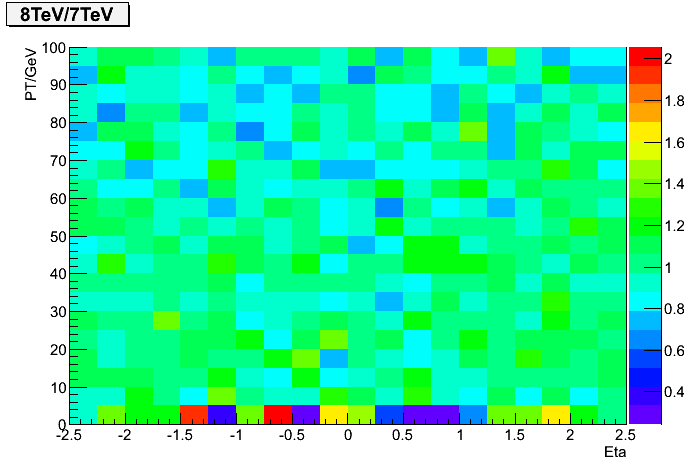
\includegraphics[width=0.55\textwidth]{plots/signal_reweight/ratio_180.png}
%%    \caption{ Ratio of 8TeV/7TeV. }
%%    \label{fig:8TeV7TeVratio}}
%%\end{figure}
%%%higgs
%%\begin{figure}[h!t]
%%  {\centering
%%    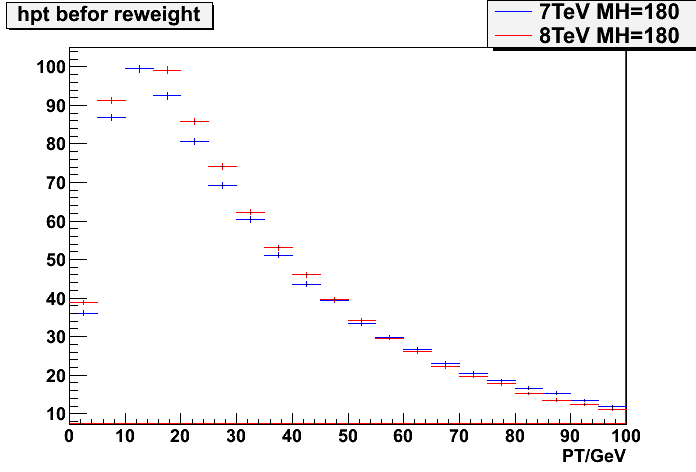
\includegraphics[width=0.49\textwidth]{plots/signal_reweight/Plots/hpt_nw.png}
%%    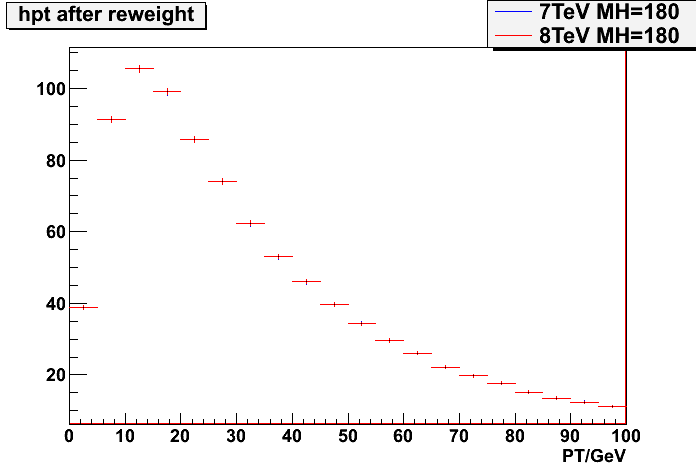
\includegraphics[width=0.49\textwidth]{plots/signal_reweight/Plots/hpt.png}
%%    \caption{Comparison of higgs pt, before and after reweighting.}
%%    \label{fig:higgspt}}
%%\end{figure}
%%\begin{figure}[h!t]
%%  {\centering
%%    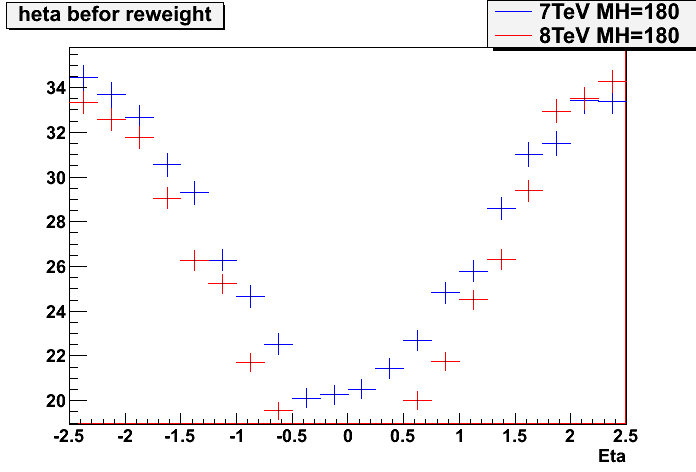
\includegraphics[width=0.49\textwidth]{plots/signal_reweight/Plots/heta_nw.png}
%%    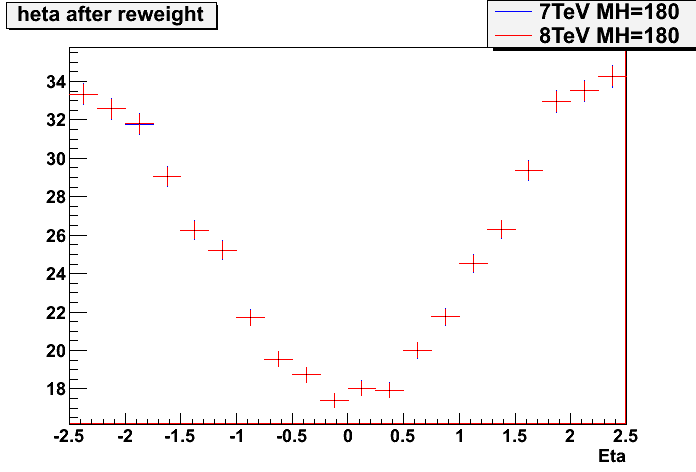
\includegraphics[width=0.49\textwidth]{plots/signal_reweight/Plots/heta.png}
%%    \caption{Comparison of higgs eta, before and after reweighting.}
%%    \label{fig:higgseta}}
%%\end{figure}
%%\begin{figure}[h!t]
%%  {\centering
%%    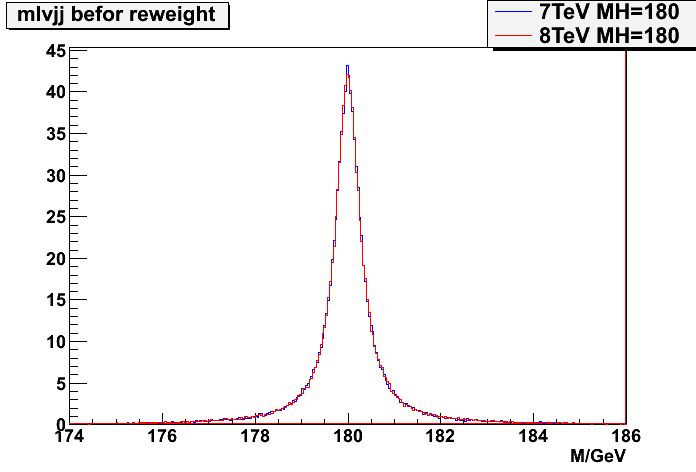
\includegraphics[width=0.49\textwidth]{plots/signal_reweight/Plots/mlvjj_nw.png}
%%    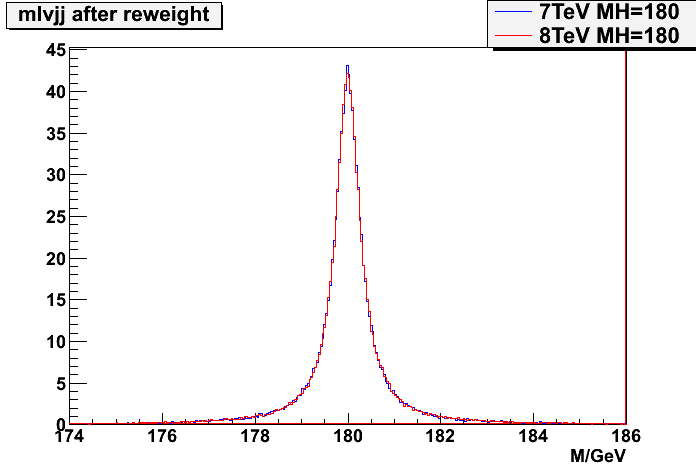
\includegraphics[width=0.49\textwidth]{plots/signal_reweight/Plots/mlvjj.png}
%%    \caption{Comparison of four body mass, before and after reweighting. The lvjj mass was reconstructed by adding the lepton, the nutrino, and the 2 jets decayed by higgs.}
%%    \label{fig:fourbodymass}}
%%\end{figure}
%%
%%%wplus
%%\begin{figure}[h!t]
%%  {\centering
%%    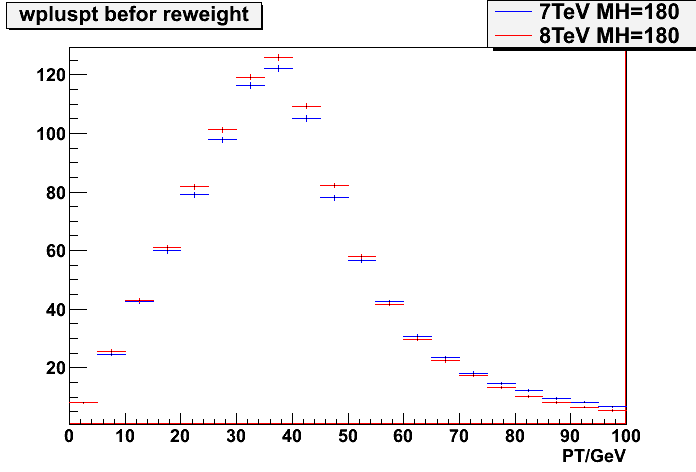
\includegraphics[width=0.49\textwidth]{plots/signal_reweight/Plots/wpluspt_nw.png}
%%    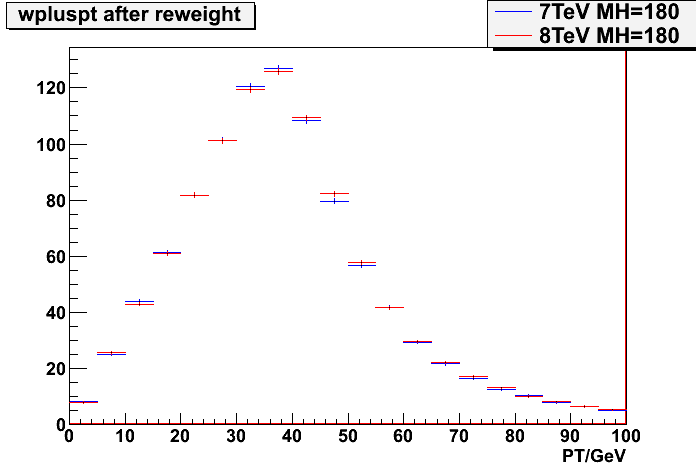
\includegraphics[width=0.49\textwidth]{plots/signal_reweight/Plots/wpluspt.png}
%%    \caption{Comparison of wplus pt, before and after reweighting.}
%%    \label{fig:wpluspt}}
%%\end{figure}
%%\begin{figure}[h!t]
%%  {\centering
%%    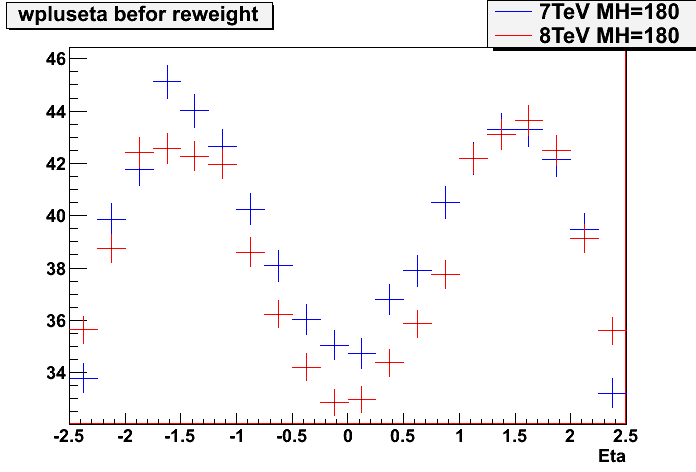
\includegraphics[width=0.49\textwidth]{plots/signal_reweight/Plots/wpluseta_nw.png}
%%    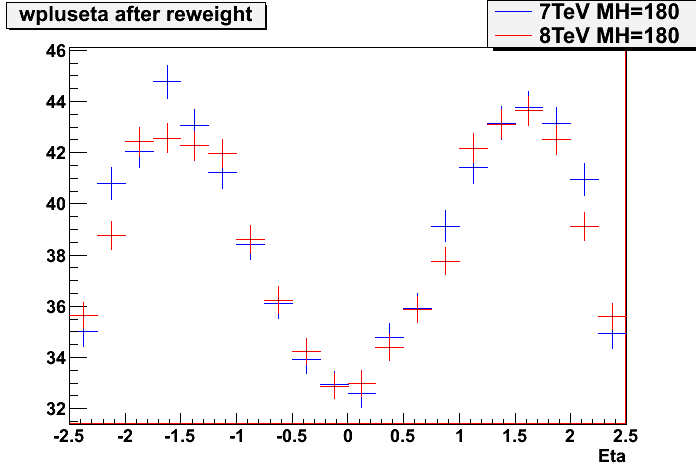
\includegraphics[width=0.49\textwidth]{plots/signal_reweight/Plots/wpluseta.png}
%%    \caption{Comparison of wplus eta, before and after reweighting.}
%%    \label{fig:wpluseta}}
%%\end{figure}
%%%wminus
%%\begin{figure}[h!t]
%%  {\centering
%%    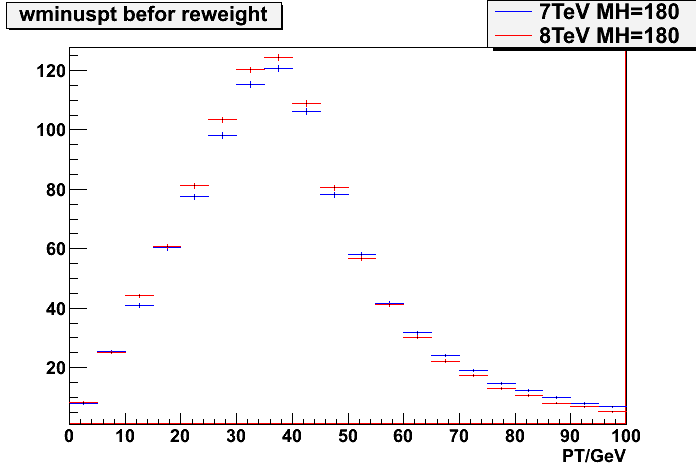
\includegraphics[width=0.49\textwidth]{plots/signal_reweight/Plots/wminuspt_nw.png}
%%    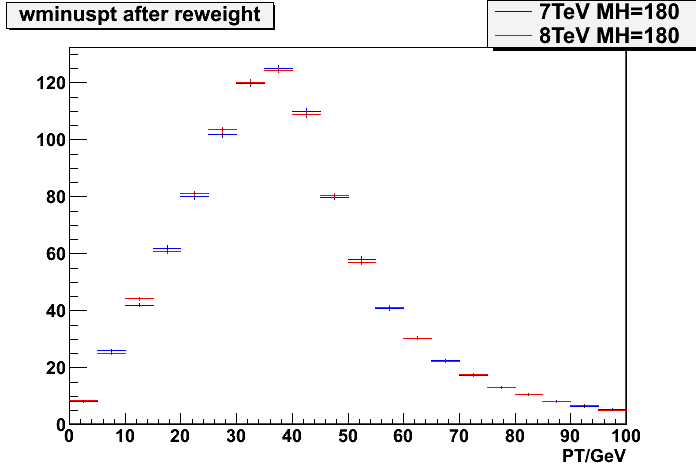
\includegraphics[width=0.49\textwidth]{plots/signal_reweight/Plots/wminuspt.png}
%%    \caption{Comparison of wminus pt, before and after reweighting.}
%%    \label{fig:wminuspt}}
%%\end{figure}
%%\begin{figure}[h!t]
%%  {\centering
%%    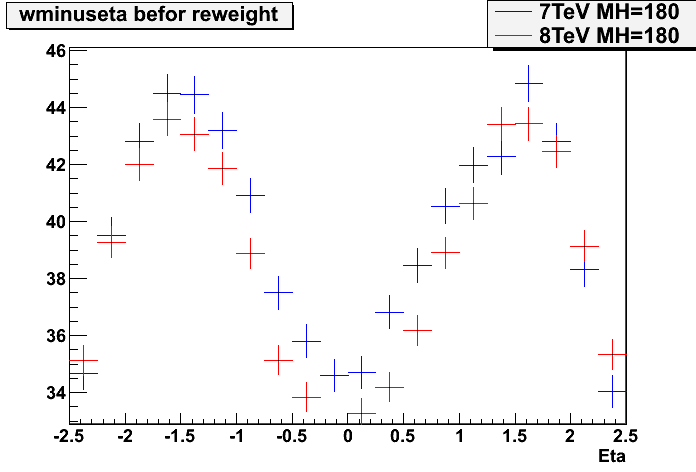
\includegraphics[width=0.49\textwidth]{plots/signal_reweight/Plots/wminuseta_nw.png}
%%    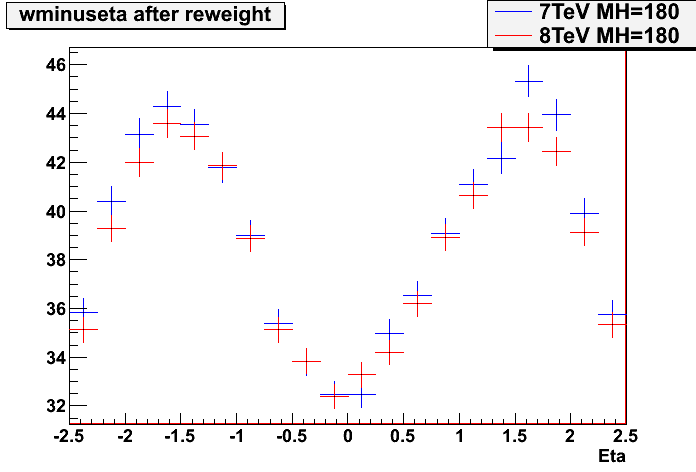
\includegraphics[width=0.49\textwidth]{plots/signal_reweight/Plots/wminuseta.png}
%%    \caption{Comparison of wminus eta, before and after reweighting.}
%%    \label{fig:wminuseta}}
%%\end{figure}
%%
%%%ele
%%\begin{figure}[h!t]
%%  {\centering
%%    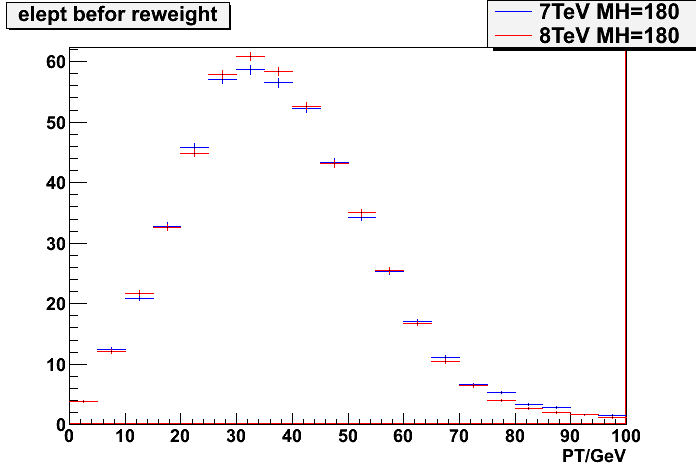
\includegraphics[width=0.49\textwidth]{plots/signal_reweight/Plots/elept_nw.png}
%%    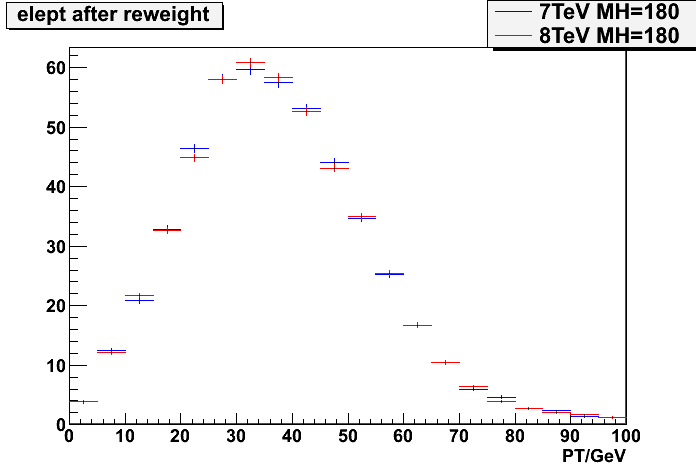
\includegraphics[width=0.49\textwidth]{plots/signal_reweight/Plots/elept.png}
%%    \caption{Comparison of electron pt, before and after reweighting.}
%%    \label{fig:electronpt}}
%%\end{figure}
%%\begin{figure}[h!t]
%%  {\centering
%%    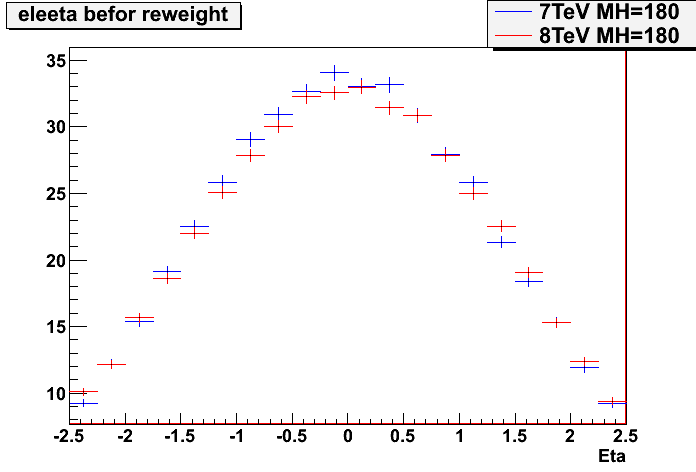
\includegraphics[width=0.49\textwidth]{plots/signal_reweight/Plots/eleeta_nw.png}
%%    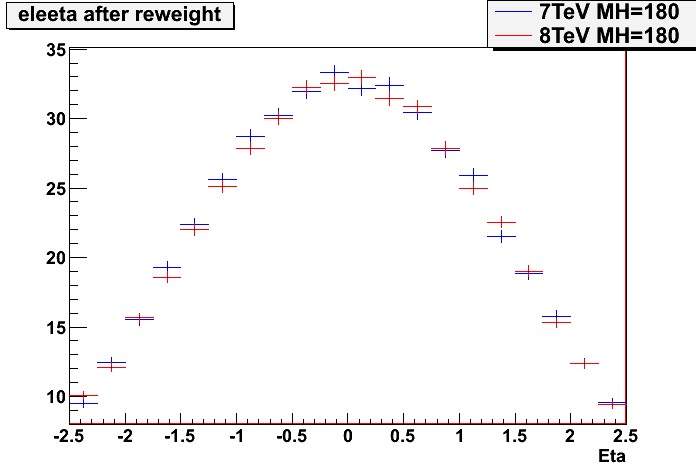
\includegraphics[width=0.49\textwidth]{plots/signal_reweight/Plots/eleeta.png}
%%    \caption{Comparison of elctron eta, before and after reweighting.}
%%    \label{fig:elctroneta}}
%%\end{figure}
%%%mu
%%\begin{figure}[h!t]
%%  {\centering
%%    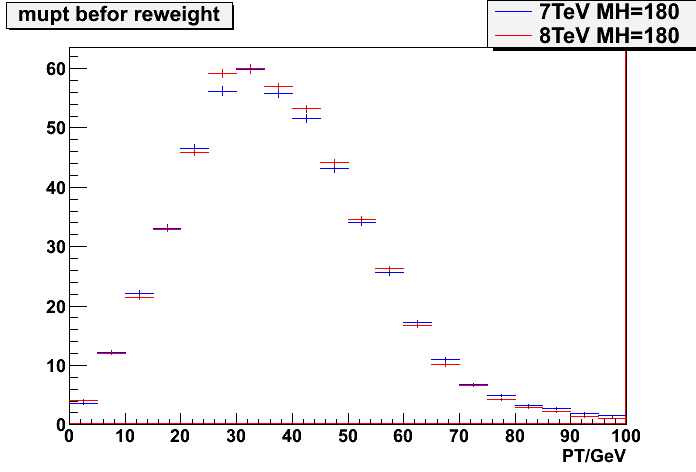
\includegraphics[width=0.49\textwidth]{plots/signal_reweight/Plots/mupt_nw.png}
%%    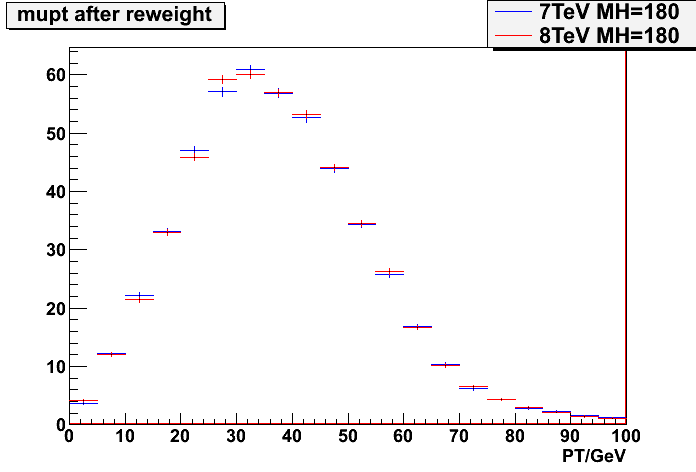
\includegraphics[width=0.49\textwidth]{plots/signal_reweight/Plots/mupt.png}
%%    \caption{Comparison of muon pt, before and after reweighting.}
%%    \label{fig:muonpt}}
%%\end{figure}
%%\begin{figure}[h!t]
%%  {\centering
%%    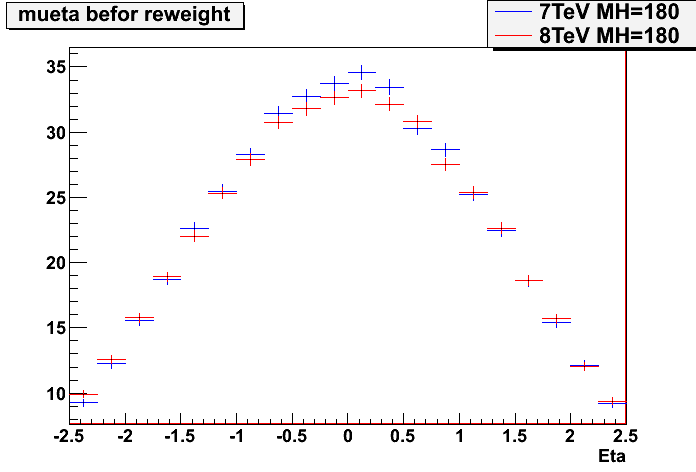
\includegraphics[width=0.49\textwidth]{plots/signal_reweight/Plots/mueta_nw.png}
%%    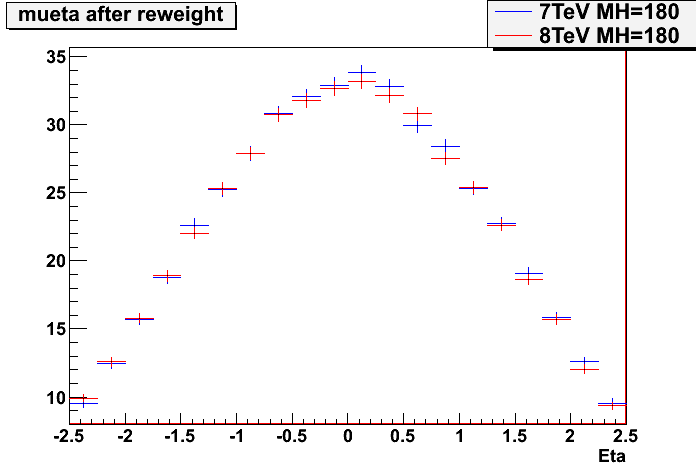
\includegraphics[width=0.49\textwidth]{plots/signal_reweight/Plots/mueta.png}
%%    \caption{Comparison of muon eta, before and after reweighting.}
%%    \label{fig:muoneta}}
%%\end{figure}
%%%jet
%%\begin{figure}[h!t]
%%  {\centering
%%    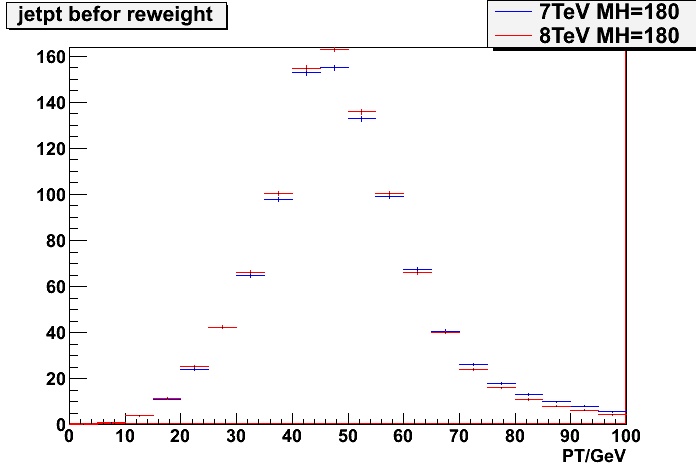
\includegraphics[width=0.49\textwidth]{plots/signal_reweight/Plots/jetpt_nw.png}
%%    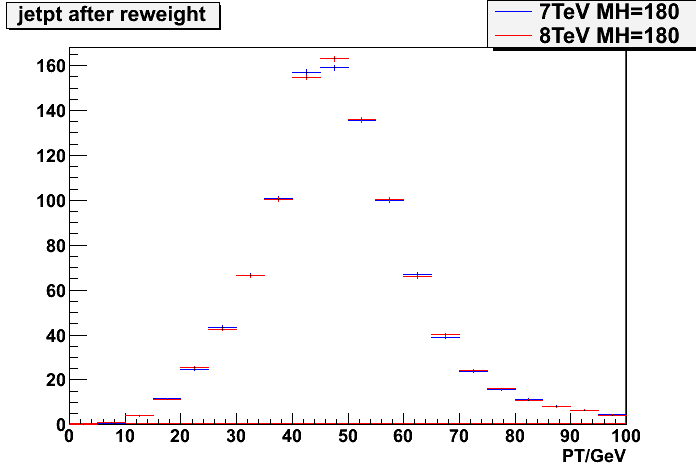
\includegraphics[width=0.49\textwidth]{plots/signal_reweight/Plots/jetpt.png}
%%    \caption{Comparison of leading jet pt, before and after reweighting.}
%%    \label{fig:leadingjetpt}}
%%\end{figure}
%%\begin{figure}[h!t]
%%  {\centering
%%    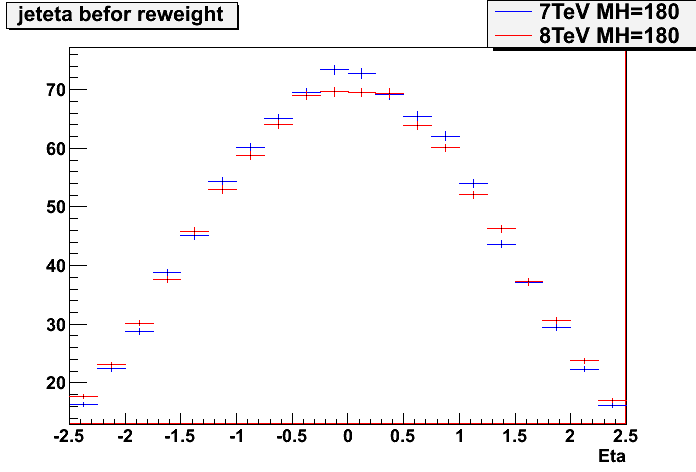
\includegraphics[width=0.49\textwidth]{plots/signal_reweight/Plots/jeteta_nw.png}
%%    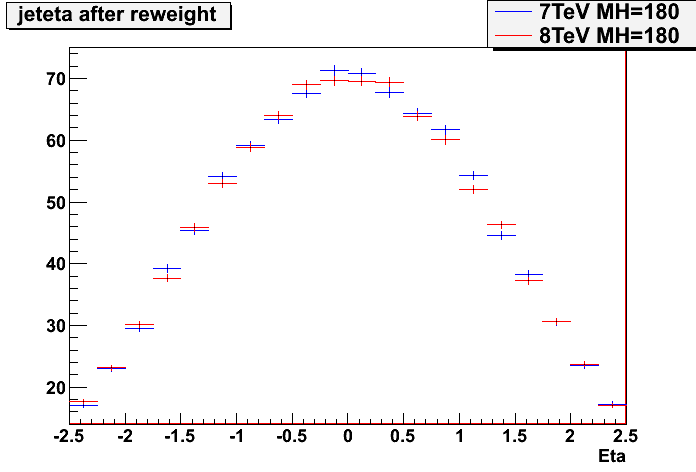
\includegraphics[width=0.49\textwidth]{plots/signal_reweight/Plots/jeteta.png}
%%    \caption{Comparison of leading jet eta, before and after reweighting.}
%%    \label{fig:leadingjeteta}}
%%\end{figure}
%%%nutrino
%%\begin{figure}[h!t]
%%  {\centering
%%    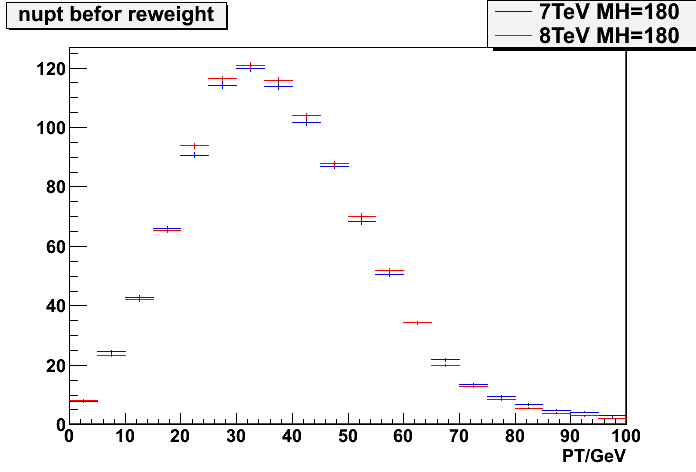
\includegraphics[width=0.49\textwidth]{plots/signal_reweight/Plots/nupt_nw.png}
%%    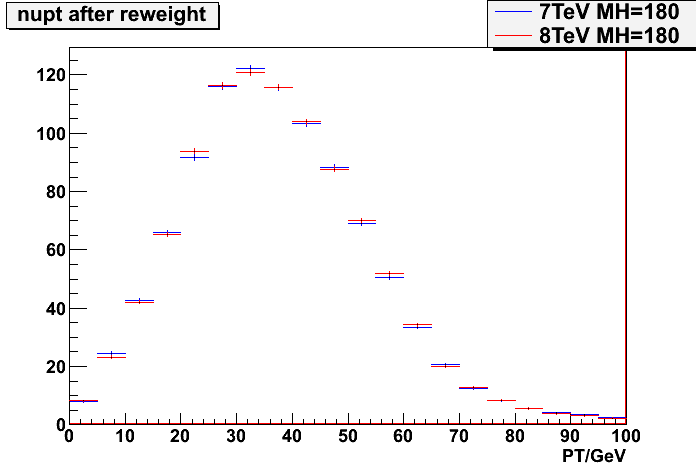
\includegraphics[width=0.49\textwidth]{plots/signal_reweight/Plots/nupt.png}
%%    \caption{Comparison of nutrino pt, before and after reweighting.}
%%    \label{fig:nutrinopt}}
%%\end{figure}
%%
%%%\begin{figure}[h!t]
%%%  {\centering
%%%    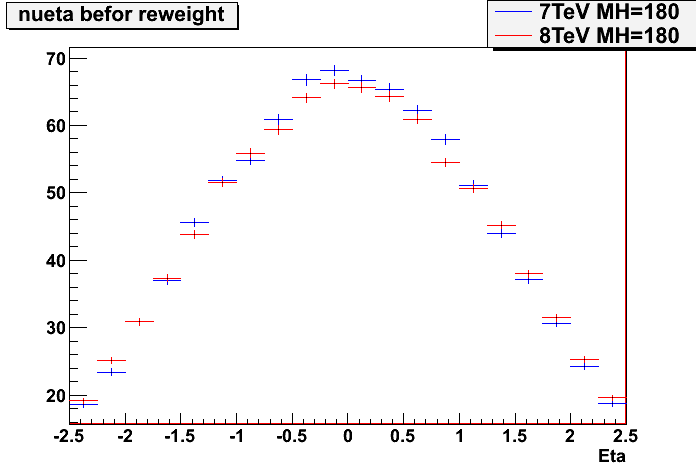
\includegraphics[width=0.49\textwidth]{plots/signal_reweight/Plots/nueta_nw.png}
%%%    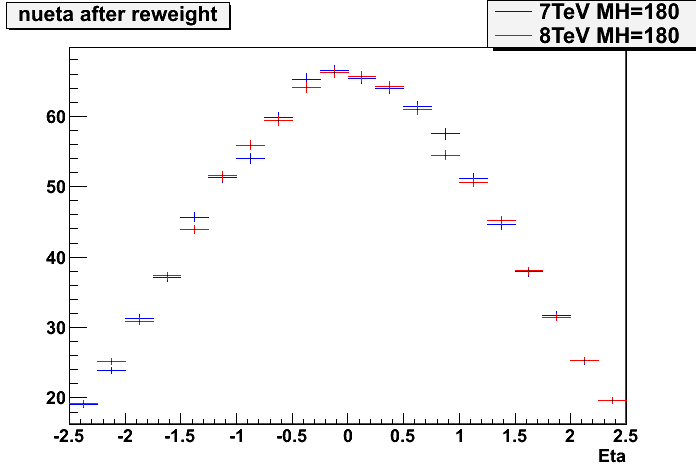
\includegraphics[width=0.49\textwidth]{plots/signal_reweight/Plots/nueta.png}
%%%    \caption{Comparison of nutrino eta, before and after reweighting.}
%%%    \label{fig:nutrino eta}}
%%%\end{figure}


\clearpage
